\documentclass{astroedu-lab}

\begin{document}

\pagestyle{plain}

\begin{problem}{\large Лабораторная работа 1.2.4}

\begin{bfseries}
	Задание:
\end{bfseries}

Определение главных моментов инерции твердых тел с помощью крутильных колебаний.

\begin{bfseries}
	Цель работы:
\end{bfseries}

Измерить периоды крутильных колебаний рамки при различных положениях закрепленного в ней тела, проверить теоретическую зависимость между периодами крутильных колебаний тела относительно различных осей, определить моменты инерции относительно нескольких осей для каждого тела, по ним найти главные моменты инерции тел и построить эллипсоид инерции.

\begin{bfseries}
	В работе используются:
\end{bfseries}

Установка для получения крутильных колебаний (жесткая рамка, имеющая винты для закрепления в ней твердых тел, подвешенная на натянутой вертикально проволоке), набор исследуемых твердых тел, секундомер.

\begin{bfseries}
	Решение:
\end{bfseries}

\begin{bfseries}
	Теоретическая справка
\end{bfseries}

Инерционные свойства твердого тела при вралцении определяет не
только величина его массы, но и ее пространственное распределение.
Последнее характеризует физическая величина, которая называется
тензором инерции.

Тензор инерции твердого тела может быть представлен симметричной матрицей, которая полностью определяется заданием шести элементов. Поэтому матрица тензора инерции может быть приведена к диагональному виду, элементы которой называются главными моментами инерции тела. Геометрическим образом тензора инерции является эллипсоид, уравнение которого в главных осях имеет вид:

\begin{equation}
	I_x x^2 + I_y y^2 + I_z z^2 = 1
\end{equation}


Этот эллипсоид принято называть эллипсоидом инерции. Эллипсоид
инерции жестко связан с телом, для которого построен. Координатные оси Ох Оу Оz совпадают с главными осями тела. Если начало
координат О совпадает с центром масс тела, то эллиисоид инерции
называется центральным.

По полученному эллипсоиду инерции можно найти момент инерции относительно любой оси, проходящей через центр эллипсоида. Для этого необходимо вдоль выбранной оси провести радиус-вектор $\overrightarrow{r}$ до пересечения с поверхностью эллипсоида. Длина r будет определять искомый момент инерции.

Главные оси тела часто можно определить из его симметрии. Эллипсоид инерции оказывается симметричным и для некоторых тел, не обладающих осевой симметрией. Например для куба эллипсоид превращается в сферическую поверхность, из чего следует, что величина момента инерции не зависит от направления оси. На рисунке снизу схематично изображены эллипсоиды для куба и параллелепипида.

\begin{center}
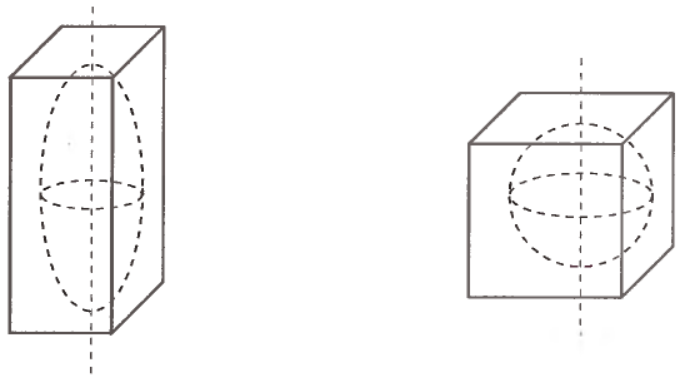
\includegraphics[width=0.7\linewidth]{rect_cube.png}
\end{center}

Для исследования момента инерции относительно разных осей используется приведенная ниже установка, которая позволяет закрепить тело в различных положениях относительно вертикали.

\begin{center}
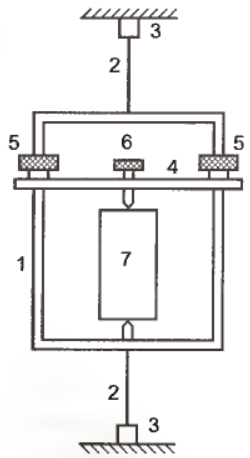
\includegraphics[width=0.25\linewidth]{device.png}
\end{center}

Крутильные колебания рамки с телом описываются уравнением гармонических колебаний

\begin{equation}
	\left(I + I_p \right) \frac{d^2 \phi}{dt^2} = - f \phi
\end{equation}

Здесь $I$ и $I_p$  - моменты инерции тела и рамки относительно оси вращения, $\phi$ - угол поворота рамки, меняющийся со временем $t$, $f$ - модуль кручения проволки.

Период крутильных колебаний системы определяется формулой

\begin{equation}
	T = 2 \pi \sqrt{\frac{I + I_p}{f}}
\end{equation}

\begin{center}
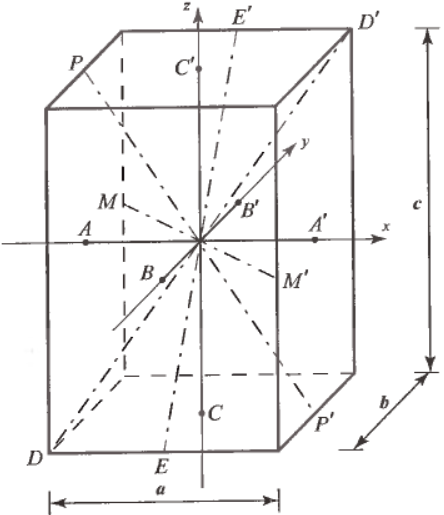
\includegraphics[width=0.5\linewidth]{scheme.png}
\end{center}

\begin{center}
\begin{tabular}[t]{|l|l|l|l|}
\hline
№ Пульки & m, г & $\Delta x$, мм & u, м/с \\
\hline
1 & 0.5030 & 11.9 & $(146 \pm 4)$ \\
2 & 0.4958 & 11.6 & $(144 \pm 4)$ \\
3 & 0.4981 & 12.2 & $(151 \pm 4)$ \\
4 & 0.5080 & 12.2 & $(148 \pm 4)$ \\
\hline
\end{tabular}
\end{center}



\end{problem}
\end{document}